\subsection{Memory Design for Accelerator Systems}

%Each DRAM memory channel comprises of several ranks. Each of these ranks is further subdivided logically into independent memory arrays called banks, each having several rows. Each row can hold a page of memory(2-4KB). 
In a DRAM cell, the data is retained for only as long as the capacitor can hold the charge injected into it during a write operation and as a result, the data in each cell needs to be refreshed periodically. A refresh operation simply involves reading a row of data and writing it back from the sense amplifier. The memory controller periodically issues commands at rank-level granularity to refresh each rank. A refresh controller keeps track of the address of the last row to have been refreshed so that the subsequent refresh command can enable it to issue refreshes to the next group of rows.
According to JEDEC SDRAM standards~\cite{jedec-sdram-standards}, a DRAM device can issue a maximum of 8192 refresh commands within a 64~ms refresh window, leading to a refresh command being issued every 7.8$\mu$s ($t_{REFI}$). The major drawback of DRAM is the additional overhead in performance and power on account of the refresh operation. A single refresh command to a row causes the entire bank of the DRAM to stall. Hence several techniques have been incorporated into the DDR protocols to minimize overlaps between read/write and refresh commands. Figure~\ref{fig:refreshTrends}a) shows the increasing nature of the JDEC parameter $t_{RFC}$ - the amount of time that each refresh locks up the DRAM - across different DRAM densities. As an example of the impact, Figure~\ref{fig:refreshTrends}b) shows energy consumption during various kernel-based computations across various DRAM generations. The refresh component in the DRAM is becoming a major source of concern with increasing DRAM densities. Each refresh command issued by the memory controller is appended to the command queue along with other read and write commands.  
Considerable work has gone into the area of reducing refresh power consumptions. Some have used scheduling policies~\cite{Stuecheli2010}, some have used retention profiling~\cite{Liu2012}, while others have used software techniques~\cite{Liu2012}. In~\cite{Nair2013}, the authors use a refresh pausing mechanism to exploit idle cycles in memory. In~\cite{Mukundan2013}, Fine Grained Refresh (FGR) for DDR4 DRAM systems is analyzed. 
However, most of these schemes are for a general purpose multicore system and are not geared to exploit the data-specific aspects prevalent in our system. 
%Therefore there is great potential for exploiting this data-related information for optimizing memory performance and energy in these vision-based accelerator systems.

%\begin{figure}[ht!]
%\centering
%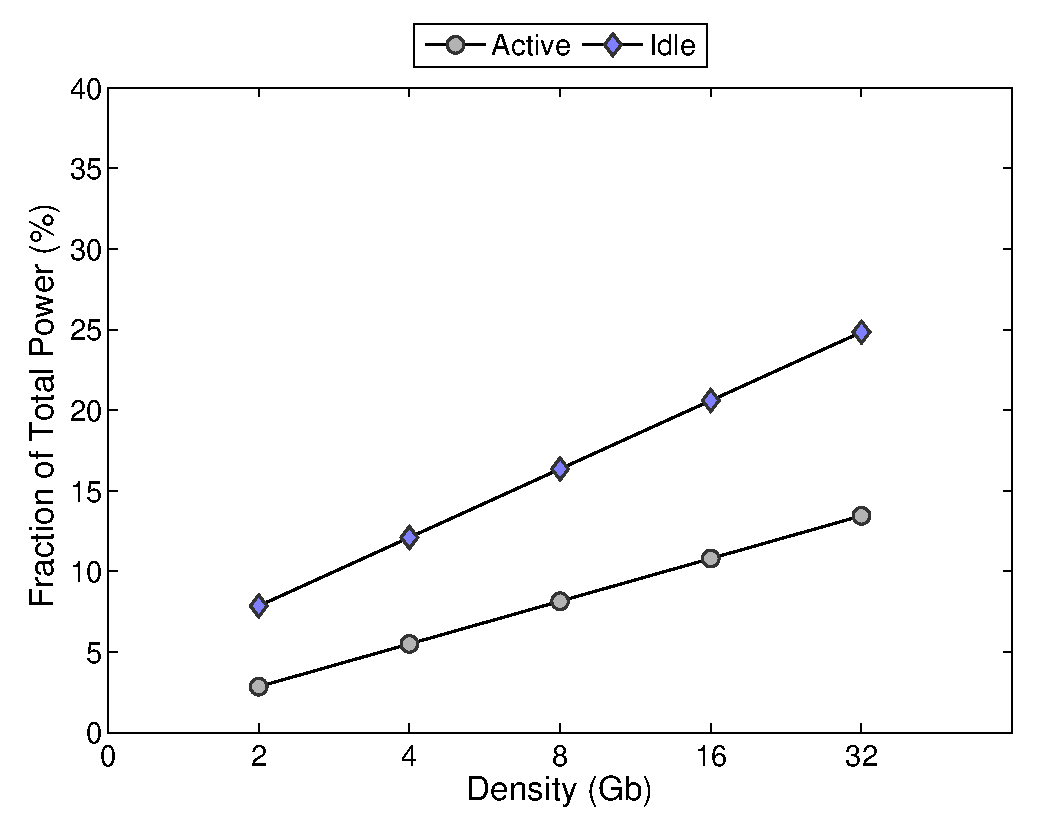
\epsfig{file=figs/RefreshTrends.eps, angle=0, width=1\linewidth, clip=}
%\caption{\label{fig:refreshTrends} Trends in the distribution of DRAM power- The refresh component increases with each generation.}
%\end{figure}

\begin{figure}[ht!]
\begin{minipage}[b]{1\linewidth}
\centering
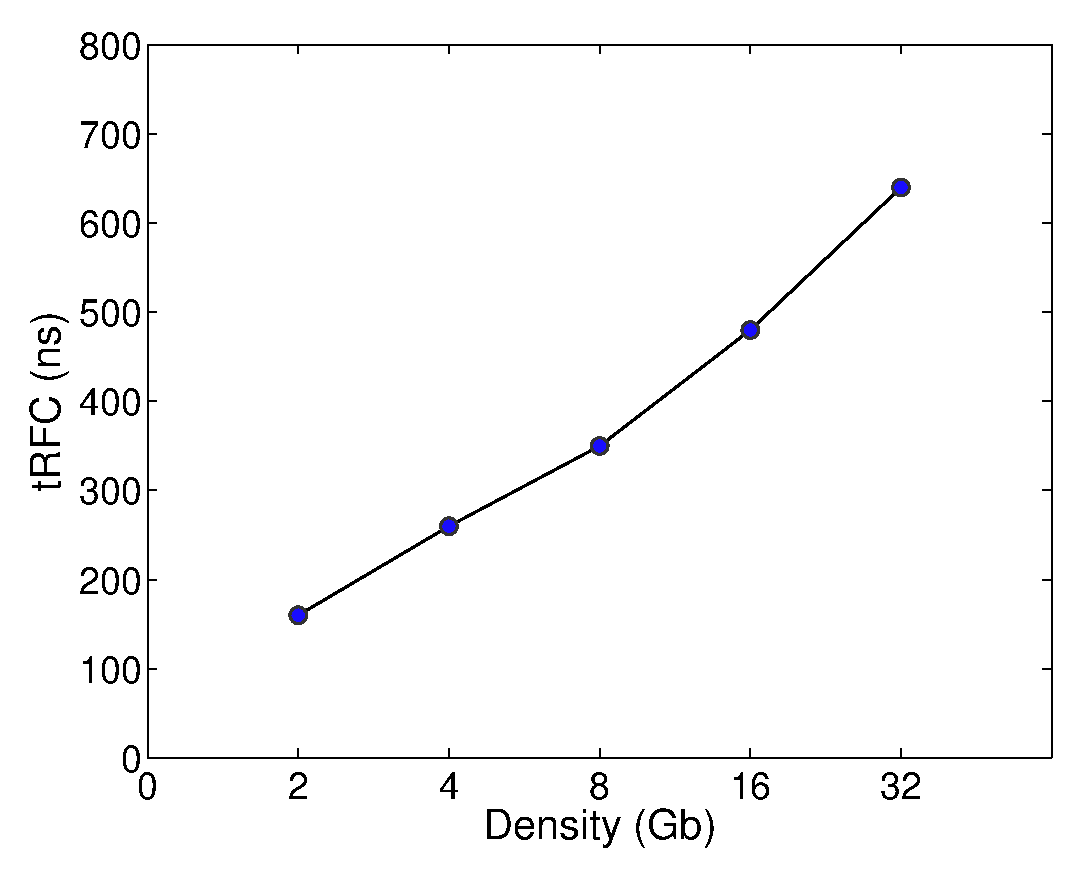
\epsfig{file=figs/tRFC.eps, angle=0,  height=0.45\linewidth, width=0.95\linewidth, clip=}
\caption{\label{fig:refreshTrends}a) The REF command time (tRFC) parameter is increasing with each generation~\cite{jedec-sdram-standards}. The values for 16 Gb and 32 Gb devices are based on projections.}
\vspace{0.1in}
\end{minipage}
\addtocounter{figure}{-1}
\begin{minipage}[b]{1\linewidth}
\centering
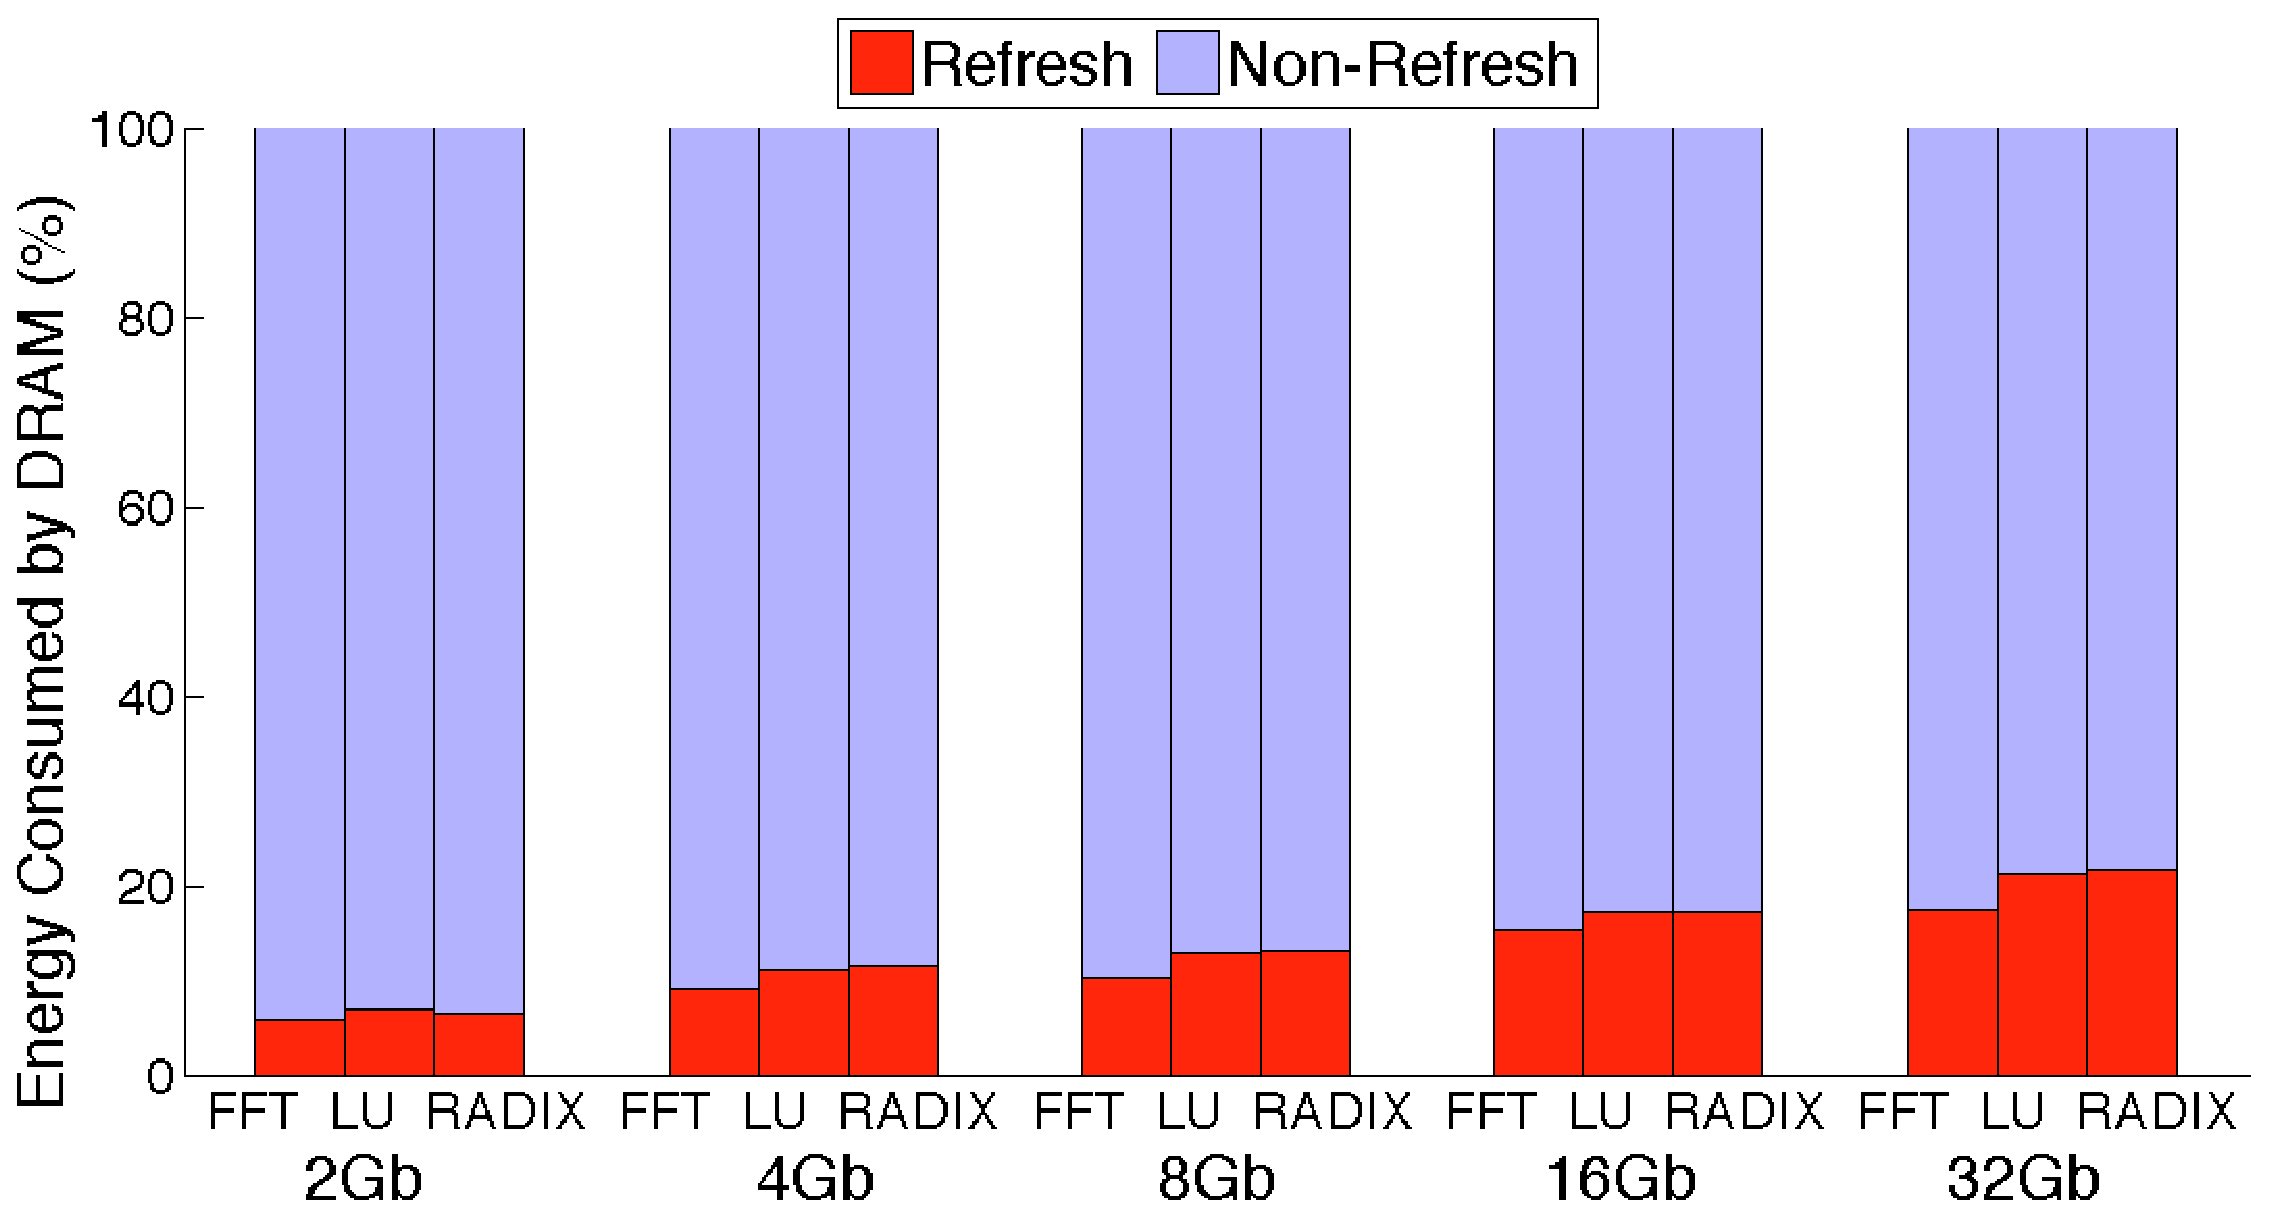
\epsfig{file=figs/DRAMEnergy_Kernels.eps, angle=0, height=0.4\linewidth, width=0.95\linewidth, clip=}
\caption{\label{fig:refreshTrends}b) Refresh energy distribution in Kernel computations}
\end{minipage}
\vspace{-0.2in}
\end{figure}

